
\section{Empirical Age and Metallicity Gradients}
\label{outflows:sec:empirical}
There are many spectroscopic surveys to choose from to characterize the age and
abundance structure of the MW, such as LAMOST~\citep{Luo2015},
GALAH~\citep{DeSilva2015, Martell2017},~\gaia-ESO~\citep{Gilmore2012}, and
APOGEE\space\citep{Majewski2017}.
APOGEE provides excellent coverage of the Galactic disk by targeting luminous
evolved stars accessible at large distances, making it particularly well-suited
for this task.
It is also less susceptible to dust obscuration since its spectra are at
near-IR wavelengths ($\lambda = 1.51 - 1.70~\mu$m;~\citealt{Wilson2019}).

% APOGEE is particularly well suited to this task, because it targets luminous
% evolved stars accessible at large distances and observes them at near-IR
% wavelengths, which are less susceptible to dust obscuration.
% Using the 2.5 m Sloan Foundation Telescope~\citep{Gunn2006} and the 2.5 m
% du Pont Telescope~\citep{Bowen1973} at Las Campanas Observatory, APOGEE
% collects high-resolution spectra between~$1.51$ and~$1.70~\mu$m
% ($R \approx 22,500$;~\citealp{Wilson2019}) of stars on a grid of sightlines at
% Galactic latitudes of~$b = 0$,~$\pm 4^\circ$, and~$\pm 8^\circ$ (targeting is
% described in detail by~\citealt{Zasowski2013, Zasowski2017, Beaton2021}, and
% \citealt{Santana2021}).
% After reduction and calibration with the APOGEE data processing pipeline
% \citep{Nidever2015}, stellar parameters such as~$T_\text{eff}$,~$\log g$, and
% abundances of 15 or more elements per target are then computed using the APOGEE
% Stellar Parameters and Chemical Abundances
% Pipeline~\citep[ASPCAP;][]{Holtzman2015, GarciaPerez2016}.

\subsection{The Sample}
\label{outflows:sec:empirical:apogee}
In this chapter, we use the~\textsc{AstroNN} value added catalog\footnote{
	\url{https://www.sdss.org/dr18/data_access/value-added-catalogs/?vac_id=85}
} for APOGEE's seventeenth data release~\citep[DR17;][]{Abdurrouf2022}.
In constructing the original catalog,~\citet{Mackereth2019b} used
\textsc{AstroNN}~\citep{Leung2019a} to train a Bayesian convolutional neural
network on APOGEE DR14 spectra and asteroseismic data from APOKASC-2
\citep{Pinsonneault2018}.
Retrained on APOGEE DR17 spectra, the value added catalog improves the
performance at low metallicity by incorporating asteroseismic ages from
\citet{Montalban2021} and additionally provides individual stellar abundances
\citep{Leung2019a} and distances~\citep{Leung2019b} retrained
with~\gaia-eDR3~\citep{GaiaCollaboration2021}.
We filter the sample based on the following selection criteria:
\begin{itemize}

	\item \texttt{STAR\_BAD == 0}

	\item \texttt{EXTRATARG == 0}

	\item S/N~$\geq 80$

	\item $\log g = 1 - 3.8$

	\item $T_\text{eff} = 3500 - 5500$ K

\end{itemize}
To avoid potential contamination by the main sequence, we additionally exclude
stars with surface gravities of~$\log g > 3$ and effective temperatures of
$T_\text{eff} < 4000$ K.
These cuts yield a final sample of 191,173 red giant and red clump stars.

\begin{figure}
\centering
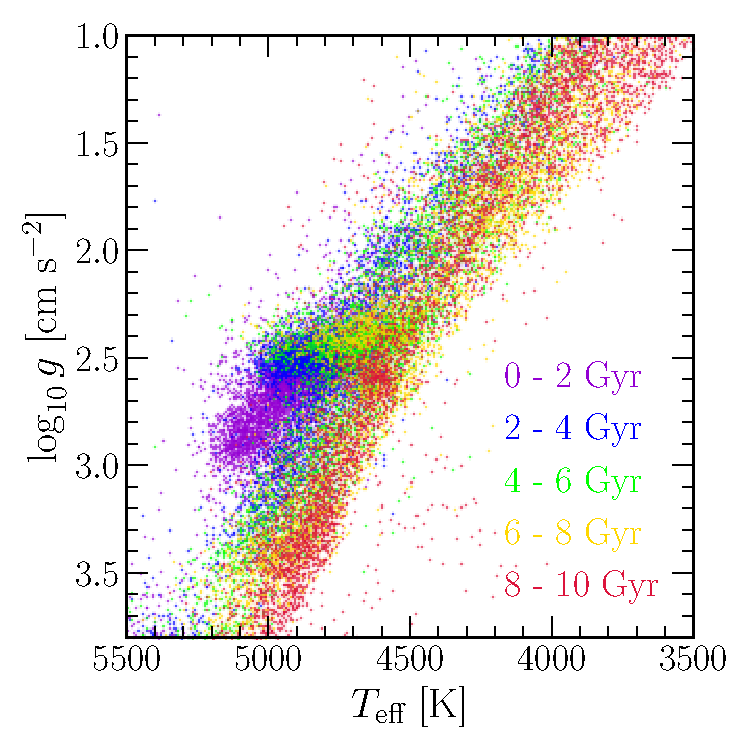
\includegraphics[scale = 0.6]{kiel_diagram.pdf}
\caption{
The Kiel diagram of our sample, color-coded by stellar age according to the
legend.
Within each age bin, we plot only a random subsample of~$N = 5000$ stars.
}
\label{outflows:fig:kiel-diagram}
\end{figure}

Fig.~\ref{outflows:fig:kiel-diagram} shows the Kiel diagram of a subsample of
our stars binned by age.
Comparing the distributions of stars along the red giant branch and red clump
between age bins indicates some systematic biases present in the sample.
The youngest stars are preferentially located in the red clump, whereas the
oldest stars distribute themselves much more evenly along the red giant branch.
This result is unsurprising as systematic uncertainties in APOGEE tend to
present as spurious correlations with~$T_\text{eff}$ and~$\log g$
\citep[e.g.,][]{Joensson2018, Eilers2022}.
However, we do not expect these systematic effects to impact our
characterizations of radial age and metallicity gradients (see discussion
in~\S~\ref{outflows:sec:empirical:caveats} below).
\par
Fig.~\ref{outflows:fig:age-xh-dists} shows age and abundance distributions of
our sample in bins of Galactocentric radius.
Stars tend to be young in the outer Galaxy, where the age distributions have a
peak around~$\sim$$2-4$ Gyr and a tail toward older ages.
As radius increases, the age distribution shifts to a peak at older ages and a
skew-negative tail.
This result is a natural consequence of inside-out Galaxy formation, whereby
the inner regions of the disk assemble at high redshift and the outer regions
follow suit on longer timescales~\citep[e.g.,][]{White1991, Bird2013}.
Abundances follow a similar pattern, shifting from a metal-rich mode and
skew-negative tail to a metal-poor mode and skew-positive tail with increasing
radius (a result previously found in APOGEE by~\citealt{Hayden2015}).
These bulk shifts in stellar population properties with radius are indicative
of radial gradients, which we quantify in more detail below.

% Although there is no analytic expression for the peak, given the mean~$\mu$ and
% standard deviation~$\sigma$ of the corresponding unskewed distribution, an
% accurate numerical approximation is given by~$\mu + m_0 \sigma$, where
% \begin{equation}
% m_0 \equiv \sqrt{\frac{2}{\pi}}
% \left[
% \delta - \left(\frac{4 - \pi}{2}\right)
% \frac{\delta^3}{\pi - 2\delta^2}
% \right] - \frac{\text{sign}(a)}{2} e^{-2\pi / \left|a\right|}
% \end{equation}
% for~$\delta \equiv a / \sqrt{1 + a^2}$ defined in terms of the skewness
% parameter~$a$~\citep{Azzalini2014}.

\subsection{Radial Gradients}
\label{outflows:sec:empirical:gradients}

To quantify the gradients in our sample, we first sort stars into 1-kpc wide
bins in Galactocentric radius.
We then compute the median age~$\tau_{1/2}$ and the 16th and 84th percentiles
of the distribution by simply sorting the values into ascending order.
The left panel of Fig.~\ref{outflows:fig:gradxh-gradage} shows the results of
this procedure.
Our sample is large enough that bootstrap error estimates indicate statistical
uncertainties smaller than the points in the figure.
A linear regression indicates a median trend of~$\gradage = -0.375 \pm 0.036$
Gyr/kpc with an intercept of~$8.21 \pm 0.31$ Gyr.
The median age closely follows this line of best fit at~$R \lesssim 9$ kpc, but
flattens off in the outer disk and reverses sign slightly.

% \afterpage{
% \clearpage
\begin{landscape}
\begin{figure*}
\centering
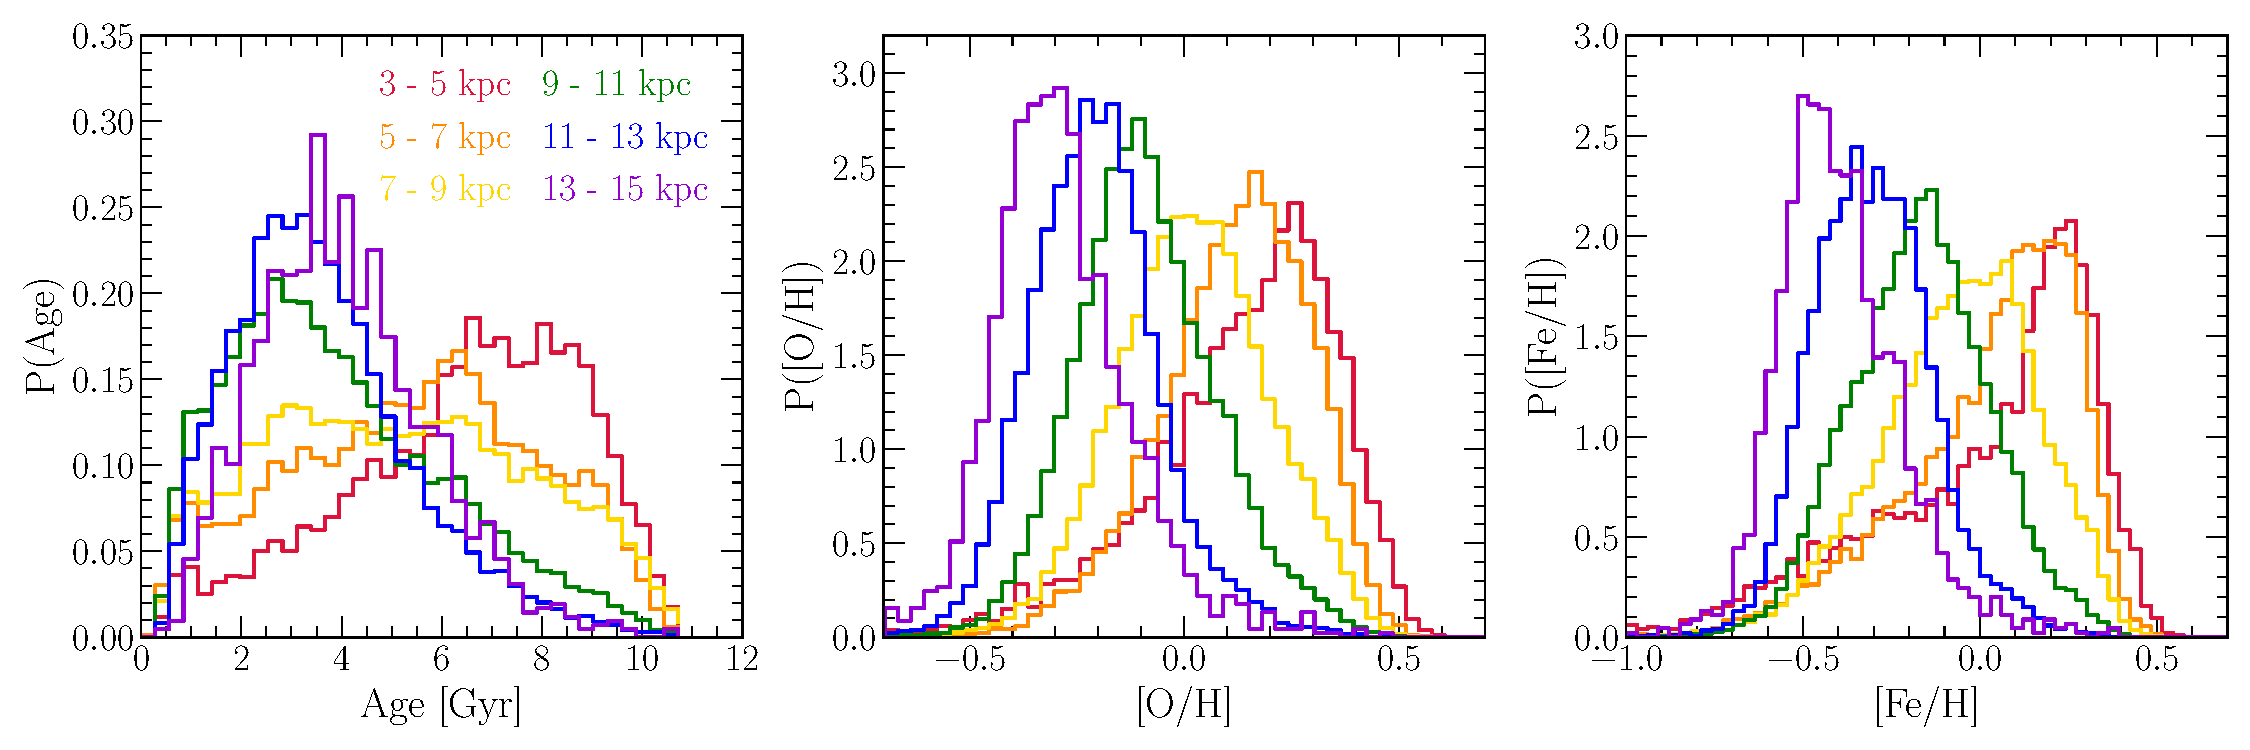
\includegraphics[scale = 0.55]{age_xh_dists.pdf}
\caption{
Age (left) and abundance (middle and right) distributions from our APOGEE
sample (see discussion in~\S~\ref{outflows:sec:empirical:apogee}) at different
radii.
Within each 2-kpc wide bin in radius, we box-car smooth the distribution with a
width of~$\Delta \tau = 1$ Gyr in age and~$\Delta$[X/H] = 0.2 for both O and
Fe.
}
\label{outflows:fig:age-xh-dists}
\end{figure*}
\end{landscape}
% \clearpage
% }

\begin{figure*}
\centering
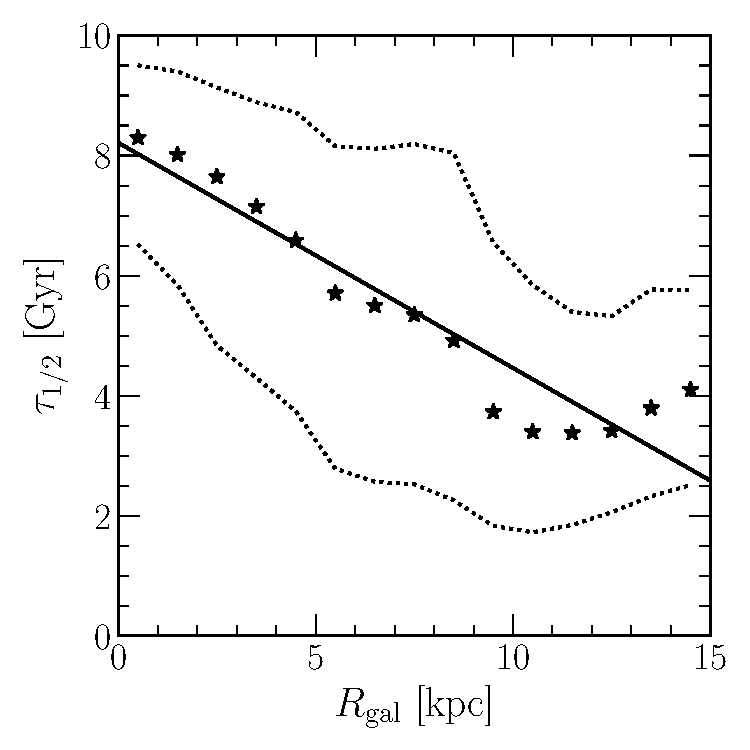
\includegraphics[scale = 0.51]{age_gradient.pdf}
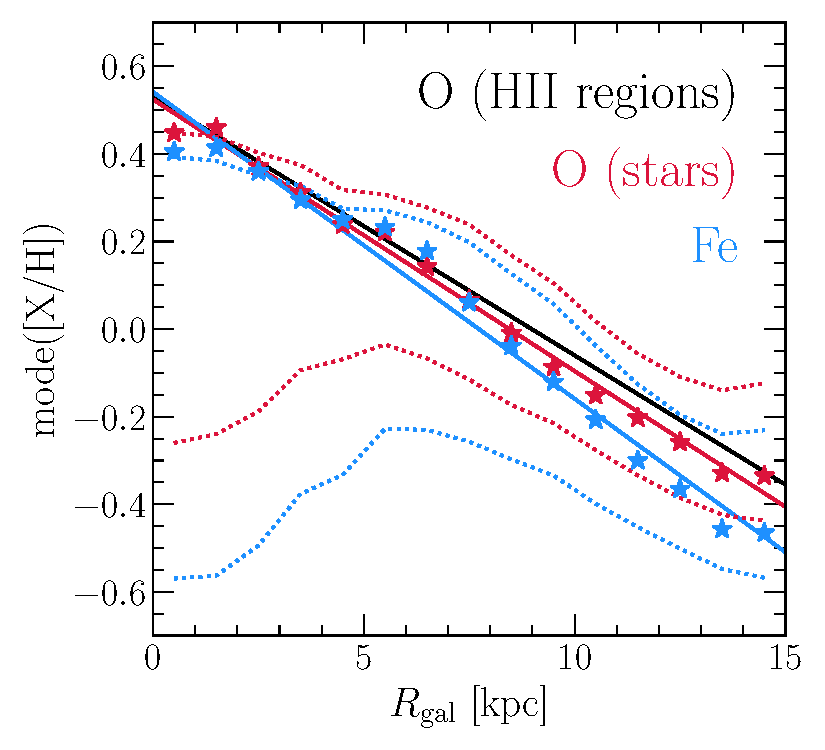
\includegraphics[scale = 0.5]{gradxh.pdf}
\caption{
Gradients in stellar age (left) and metallicity (right; red for O and blue for
Fe).
Stars denote the median age and mode abundance in 1-kpc bins of radius, with
dotted lines marking the 16th and 84th percentiles of the distributions in each
radial bin.
Solid lines denote the lines of best fit applied to the corresponding summary
statistics, with the fit parameters summaries in Table X.
The black line in the right hand panel marks the O abundance gradient in
Galactic HII regions measured by~\citet{MendezDelgado2022}.
}
\label{outflows:fig:gradxh-gradage}
\end{figure*}

Though we quantify the age gradient in terms of the median trend, the mode is
our summary statistic of choice in quantifying metallicity gradients.
We discuss our motivation behind this choice in~\S~{\color{red} X}.
In short, our GCE models suggest that the mode is not significantly affected
by stellar migration, {\color{red} except perhaps in the outermost regions of
the disk(?).}
Consequently, its variations should reflect the enrichment histories of
different Galactic regions with little contamination.
Because the mode is a noisy statistic, we fit a skewed normal distribution to
the MDF in each radial bin and determine the mode by optimization.
We however estimate the 16th and 84th percentiles by simply sorting the
abundances into ascending order as we did for the age distributions.
\par
The right panel of Fig.~\ref{outflows:fig:gradxh-gradage} shows the resultant
gradients in~\oh~and~\feh.
As expected given the MDFs in Fig.~\ref{outflows:fig:age-xh-dists}, stars tend
to decline in metallicity with increasing radius.
Linear regressions indicate slopes of~$\grad{O} = -0.062 \pm 0.001$ kpc$^{-1}$
and~$\grad{Fe} = -0.070 \pm 0.003$ kpc$^{-1}$, in reasonable agreement with
previous measurements (see discussion in~\S~\ref{outflows:sec:intro} and
references therein).
Our GCE models {\color{red} successfully(?)} reproduce the slightly steeper
slope in Fe; we describe the origin of this result in~\S~{\color{red} X}.
For comparison, we additionally plot~\citeauthor{MendezDelgado2022}'s
\citeyearpar{MendezDelgado2022} fit to the gas-phase O gradient traced by
Galactic HII regions accounting for their temperature inhomogeneities.
The two O gradients are consistent within their~$1\sigma$ uncertainties.
\par
We use these measurements to calibrate our GCE models
in~\S~\ref{outflows:sec:gce} below.
We quantify the abundance gradients conditioned on stellar age and compare
against our models in~\S~\ref{outflows:sec:results}.

\subsection{Caveats}
\label{outflows:sec:empirical:caveats}
Since our sample was produced by training~\textsc{AstroNN}'s deep learning
capabilities on APOGEE spectra, our ages may be biased by known correlations
with abundances (e.g., the age-[O/Fe] relation,~\citealt{Feuillet2019}).
To assess the impact of this decision, we have remade our measurements
in~\S\S~\ref{outflows:sec:empirical:apogee} and~\ref{outflows:sec:results}
with the~\citet{Leung2023} age catalog.
They mitigate this potential issue by compressing the spectra into lower
dimensional representations of themselves (i.e., a~\textit{latent space}) using
a variational encoder-decoder algorithm~\citep[e.g.,][]{LeCun2015}.
They then train a modified random forest algorithm to predict similarly
compressed lightcurves trained on~\textit{Kepler} photometry
\citep{Borucki2010}.
They demonstrate that this latent space contains little if any information on
chemical abundances and stellar parameters, as intended, after which they are
able to estimate ages by augmenting the latent space with~$T_\text{eff}$
and~$\log g$ and decompressing the lightcurves.
\par
We find similar results with either age catalog, indicating that any biases
introduced by abundance information in the APOGEE spectra is of little to no
concern.
Though the value added catalog exhibits a dearth of very old stars
($\gtrsim$$10$ Gyr; see Fig.~\ref{outflows:fig:age-xh-dists} and Fig. 11 of
\citealt{Leung2023}), this should not be a problem for this chapter since we
are primarily interested in~$\lesssim$$10$ Gyr old populations anyway.
The main advantage of the value added catalog over~\citet{Leung2023} is that
their ages are available only for stars with surface gravities
of~$\log g = 2.5 - 3.6$ due to their training sample.
As a result, the value added catalog is a factor of~$\sim$$2.5$ large, yielding
much more precise summary statistics.
This decision also provides better coverage of the Galactic disk as we are able
to use luminous, low-surface gravity stars on the upper red giant branch.
\par
Particularly with regard to our measurement of the age gradient, the APOGEE
selection function is a significant source of systematic uncertainty.
APOGEE primarily targets stars with 2MASS~\citep{Skrutskie2006} magnitudes
of~$7 < H < 13.8$ on a grid of sightlines at Galactic latitudes
$b = 0$,~$\pm 4^\circ$, and~$\pm 8^\circ$ (targeting is described in detail
by~\citealt{Zasowski2013, Zasowski2017, Beaton2021}, and~\citealt{Santana2021}).
Quantifying the impact of this sampling bias in APOGEE first requires relating
a star's apparent magnitude and color to a selection fraction based on its
location on the 2-D sky~\citep{Bovy2016c, Mackereth2017, Lian2022}.
One must then combine this mapping with a 3-D dust map to account for reddening
and some model of the intrinsic number density of potential targets based on
stellar properties from isochrones and an initial mass function (IMF; e.g.
\citealt{Kroupa2001, Chabrier2003}), which then results in the selection
fraction as a function of Galactic position, metallicity, and age
\citep[see also][]{Mackereth2020}.

% {\color{red} APOGEE selection function.}

% \begin{figure*}
% \centering
% 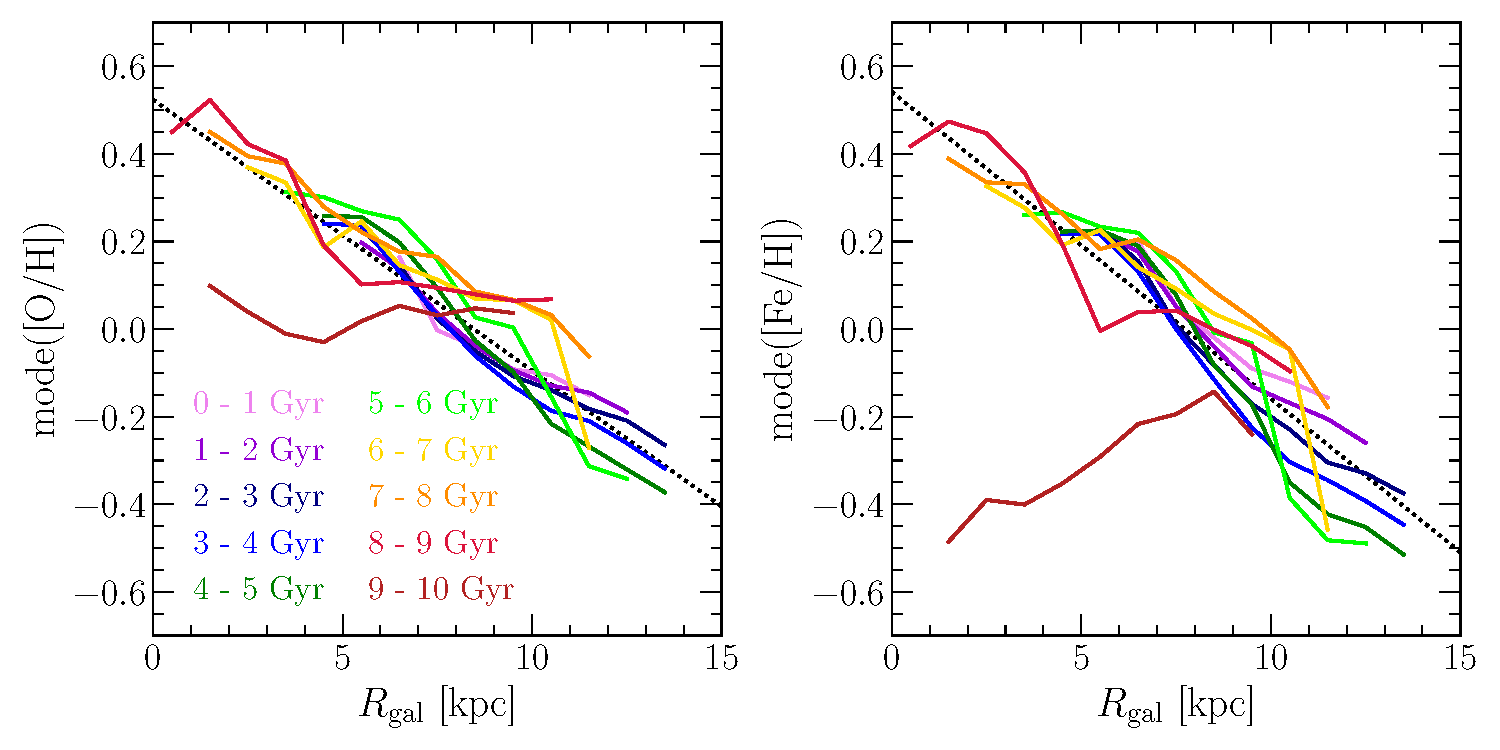
\includegraphics[scale = 0.55]{gradxh_fixedage.pdf}
% \caption{
% Radial gradients in [O/H] (left) and [Fe/H] (right) conditioned on stellar age
% in 1-Gyr bins according to the legend in the left panel.
% }
% \label{outflows:fig:gradxh-fixed-age}
% \end{figure*}

% 
{
\renewcommand{\arraystretch}{1.3}
\begin{table*}
\caption{
A summary of our linear regressions in age and metallicity gradients (see
discussion in~\S~\ref{outflows:sec:empirical:gradients}).
}
\begin{tabularx}{\columnwidth}{c @{\extracolsep{\fill}} l l l}
\toprule
Subsample & Slope & Intercept & $\chi_\text{dof}^2$
\\
\toprule
\multicolumn{4}{c}{\textbf{Age}}
\\
All Stars & $-0.375 \pm 0.036$ Gyr kpc$^{-1}$ & $8.21 \pm 0.31$ Gyr & --
\\
\midrule
\multicolumn{4}{c}{\textbf{\oh}}
\\
All Stars & $-0.062 \pm 0.001$ kpc$^{-1}$ & $0.524 \pm 0.013$ & $0.004$
\\
$0 - 1$ Gyr & $-0.055 \pm 0.011$ kpc$^{-1}$ & $0.459 \pm 0.103$ & $0.146$
\\
$1 - 2$ Gyr & $-0.056 \pm 0.005$ kpc$^{-1}$ & $0.473 \pm 0.048$ & $0.082$
\\
$2 - 3$ Gyr & $-0.059 \pm 0.005$ kpc$^{-1}$ & $0.497 \pm 0.052$ & $0.129$
\\
$3 - 4$ Gyr & $-0.066 \pm 0.004$ kpc$^{-1}$ & $0.544 \pm 0.038$ & $0.169$
\\
$4 - 5$ Gyr & $-0.079 \pm 0.004$ kpc$^{-1}$ & $0.662 \pm 0.037$ & $0.055$
\\
$5 - 6$ Gyr & $-0.080 \pm 0.007$ kpc$^{-1}$ & $0.690 \pm 0.062$ & $0.093$
\\
$6 - 7$ Gyr & $-0.055 \pm 0.008$ kpc$^{-1}$ & $0.515 \pm 0.062$ & $0.225$
\\
$7 - 8$ Gyr & $-0.049 \pm 0.002$ kpc$^{-1}$ & $0.517 \pm 0.015$ & $0.320$
\\
$8 - 9$ Gyr & $-0.049 \pm 0.007$ kpc$^{-1}$ & $0.498 \pm 0.047$ & $0.251$
\\
$9 - 10$ Gyr & $-0.001 \pm 0.005$ kpc$^{-1}$ & $0.037 \pm 0.031$ & $0.279$
\\
\midrule
\multicolumn{4}{c}{\textbf{\feh}}
\\
All Stars & $-0.070 \pm 0.003$ kpc$^{-1}$ & $0.541 \pm 0.026$ & $0.023$
\\
$0 - 1$ Gyr & $-0.068 \pm 0.010$ kpc$^{-1}$ & $0.587 \pm 0.091$ & $0.083$
\\
$1 - 2$ Gyr & $-0.072 \pm 0.005$ kpc$^{-1}$ & $0.603 \pm 0.051$ & $0.040$
\\
$2 - 3$ Gyr & $-0.077 \pm 0.006$ kpc$^{-1}$ & $0.613 \pm 0.056$ & $0.020$
\\
$3 - 4$ Gyr & $-0.083 \pm 0.005$ kpc$^{-1}$ & $0.617 \pm 0.048$ & $0.039$
\\
$4 - 5$ Gyr & $-0.096 \pm 0.007$ kpc$^{-1}$ & $0.735 \pm 0.062$ & $0.090$
\\
$5 - 6$ Gyr & $-0.097 \pm 0.012$ kpc$^{-1}$ & $0.746 \pm 0.104$ & $0.205$
\\
$6 - 7$ Gyr & $-0.066 \pm 0.012$ kpc$^{-1}$ & $0.541 \pm 0.089$ & $0.102$
\\
$7 - 8$ Gyr & $-0.051 \pm 0.004$ kpc$^{-1}$ & $0.493 \pm 0.028$ & $0.185$
\\
$8 - 9$ Gyr & $-0.061 \pm 0.008$ kpc$^{-1}$ & $0.504 \pm 0.049$ & $0.048$
\\
$9 - 10$ Gyr & $0.038 \pm 0.006$ kpc$^{-1}$ & $-0.510 \pm 0.037$ & $0.380$
\\
\bottomrule
\end{tabularx}
\label{outflows:tab:apogee-regressions}
\end{table*}
}


% \begin{figure}
% \centering
% 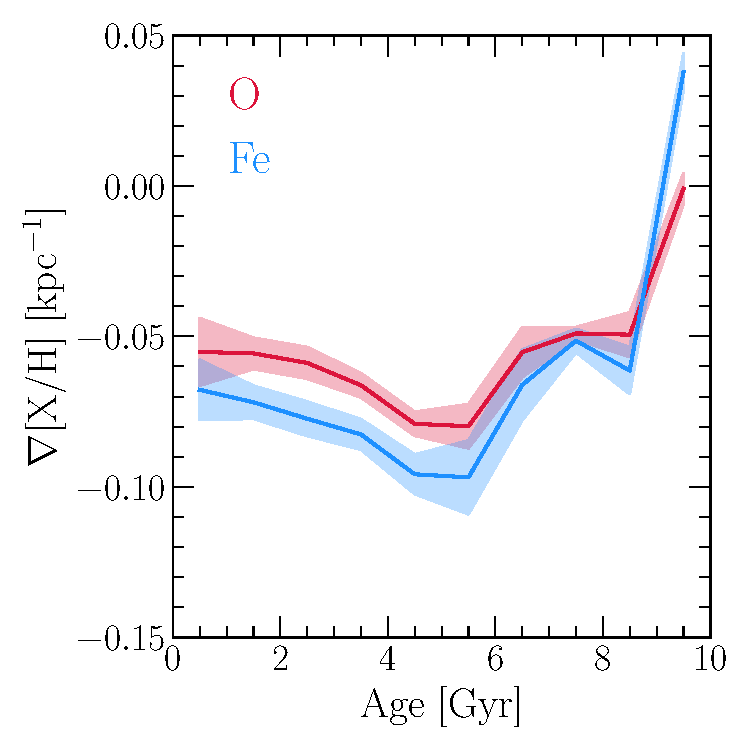
\includegraphics[scale = 0.6]{gradxh_vs_age.pdf}
% \caption{
% The slope of the radial abundance gradient in O (red) and Fe (blue) in 1-Gyr
% bins of stellar age (see discussion
% in~\S~\ref{outflows:sec:empirical:gradients}).
% }
% \label{outflows:fig:gradxh-vs-age}
% \end{figure}

% As a central interest of this chapter is to quantify the evolution of the
% Galactic abundance gradient over time, we now repeat these measurements
% conditioned on stellar age.
% In conditioning on both age and radius, we fit for the mode of the MDF only in
% bins containing at least 200 stars.
% This is a sufficiently large sample in each bin such that bootstrap resampling
% indicates statistial uncertainties in the mode comparable to the width of the
% lines plotted ($\lesssim0.1\%$).
% \par
% Fig.~\ref{outflows:fig:gradxh-fixed-age} shows the gradients themselves in each
% age bin.
% We also report slopes and intercepts from linear regressions to the trend in
% each age bin in Table~\ref{outflows:tab:apogee-regression} and visualize the
% inferred gradients in Fig.~\ref{outflows:fig:gradxh-vs-age}.
% To first order, the gradient was established~$\sim$$8 - 9$ Gyr ago.
% In the oldest age bin, the abundance profile is consistent with flat in~\oh~but
% is positively sloped in~\feh.
% The gradient held relatively steady at~$\grad{O} \approx \grad{Fe} \approx
% -0.05$ kpc$^{-1}$ for~$\sim$3 Gyr, then steepened to~$\grad{O} \approx -0.07$
% kpc$^{-1}$ and~$\grad{Fe} \approx -0.09$ kpc$^{-1}$ before gradually returning
% to~$\grad{O} \approx \grad{Fe} \approx -0.05$ kpc$^{-1}$ until the present day.
% Inspection of fig.~\ref{outflows:fig:gradxh-fixed-age} indicates that the
% steepening of the gradient coincides with a decrease in metallicity
% of~$\sim$$0.2 - 0.3$ dex in O and~$\sim$$0.4 - 0.5$ dex in Fe
% at~$R_\text{gal} \gtrsim$8 kpc.
% \par
% {\color{red} Potentially move to discussion section.}
% This result is readily explained by a dilution event due to accretion of
% metal-poor gas in the outer disk.
% A decrease in metallicity indicates that the enrichment rate and by extension
% the SFR are slow relative to the infall rate.
% A burst in star formation driven by the increased resources then naturally
% ensues~\citep[e.g.,][]{Dalcanton2007}.
% The differences in both the magnitude of the dilution in
% Fig.~\ref{outflows:fig:gradxh-fixed-age} and the timescales in
% Fig.~\ref{outflows:fig:gradxh-vs-age} between O and Fe are expected under this
% scenario.
% [O/H] and [Fe/H] decrease by the same amount only the limit that the
% accretion event is instantaneous~\citep{Johnson2020}, and O re-enrichment is
% faster due to the restitution delay of SN Ia Fe yields.

